\documentclass[12pt, a4paper, french, version=last, parskip=half, titlepage]{scrartcl}

\usepackage[a4paper, margin=2.5cm]{geometry}
\usepackage[babel, final]{microtype}
\usepackage{amssymb}
\usepackage{unicode-math}
\usepackage{mathtools}
\usepackage{babel}
\usepackage{physics}
\usepackage{siunitx}
\usepackage{booktabs}
\usepackage{multirow}
\usepackage[normalem]{ulem}
\usepackage{subcaption}
\usepackage[dvipsnames]{xcolor}
\usepackage[inline]{enumitem}
\usepackage{tcolorbox}
\usepackage{float}

% REMOVE
\usepackage[export]{adjustbox}

\makeatletter
\def\fps@figure{hptb}
\makeatother

\setmainfont{TeX Gyre Pagella}
\setsansfont{TeX Gyre Heros}
\setmathfont{TeX Gyre Pagella Math}
\setmathfont[range=\setminus]{Asana Math}

\usepackage[newfloat]{minted}
\setminted{autogobble,
           fontsize=\footnotesize,
           linenos,
           breaklines,
           xleftmargin=.7cm}

\usepackage[bookmarks,
            % hidelinks,
            breaklinks,
            pdfusetitle,
            pdfencoding=unicode]{hyperref}

% Enable \cref{...} and \Cref{...} instead of \ref
\usepackage[nameinlink, capitalize, noabbrev]{cleveref}

% \newcommand{\p}[1]{#1}
% \newcommand{\p}[1]{\mathsf{#1}}
% \newcommand{\p}[1]{\mathfrak{#1}}

\newcommand{\matlab}{\mintinline{matlab}}
\Crefname{listing}{Listing}{Listing}

\title{Systèmes de Décision \texorpdfstring{\\}{---} Projet}
\subtitle{Groupe 21}
\author{José Lucas DE MELO COSTA \and
Fernando KURIKE MATSUMOTO \and
Victor Felipe DOMINGUES DO AMARAL}
\date{Mention Intelligence Artificielle \\2021-2022}
\publishers{Université Paris-Saclay\\CentraleSupélec}

\begin{document}

\maketitle
\tableofcontents

\section{Modélisation}
\label{sec:modelisation}

\subsection{Entrées}

On peut définir $N_m$ le nombre de personnes (membres) à travailler, $N_c$ le nombre de compétences possibles, $N_p$ le nombre de projets, $N_j$ le délai maximal des projets.

L'attribution des compétences est modélisée comme $H \in \mathbb{B}^{N_m\times N_c}$
\begin{equation*}
    \text{H}_{i,k} = 
    \begin{cases}
        1, & \text{si la personne $i$ a la compétence $k$} \\
        0, & \text{sinon}
    \end{cases}
\end{equation*}

Les congés sont modélisés aussi comme une matrice $C \in \mathbb{B}^{N_m \times N_j}$
\begin{equation*}
    \text{C}_{i,\ell} = 
    \begin{cases}
        1, & \text{si la personne $i$ prends congé au jour $\ell$} \\
        0, & \text{sinon}
    \end{cases}
\end{equation*}

La nécessité des projets est modélisée comme $\text{Q} \in \mathbb{N}^{N_p \times N_c}$, avec $\text{Q}_{j,k} =  c_i$, où $c_i \in \{0, \dots, N_c\}$ est le nombre de compétences du type $k$ dont le projet $j$ a besoin.

Le revenu d'un projet $j$, $\text{Rev}_j \in \mathbb{Z}^{0+}$, est le total reçu par la réalisation de ce projet.

La pénalité d'un projet $j$, $\text{P}_j \in \mathbb{Z}^{0+}$, est le coût par jour de retard de ce projet.

La deadline d'un projet $j$, $\text{Dl}_j \in \{1, \dots, N_j\}$, est le nombre de jours accordé pour réaliser ce projet.


\subsection{Variables de décision}

Compte tenu de la modélisation du problème, nous savons que l'allocation de ressources se fera sur quatre variables : 1) la personne, 2) le projet, 3) le jour et 4) la compétence exercée. Ainsi, on utilise une variable d'optimisation binaire et de dimension égale à quatre :
\begin{equation*}
    \text{T}_{i,j,k,\ell} = 
    \begin{cases}
        1, & \text{si la personne $i$ travaille dans le projet $j$,} \\[-0.1em]
           & \text{avec la compétence $k$ au jour $\ell$} \\[0.2em]
        0, & \text{sinon}
    \end{cases}
\end{equation*}

avec $i \in \{1, \dots, N_m\}$, $j \in \{1, \dots N_p\}$, $k \in \{1, \dots, N_c\}$ et $\ell \in \{1, \dots, N_j\}$.

Nous définissons aussi des variables auxiliaires :

\begin{itemize}
    \item Une variable binaire $\text{R} \in \mathbb{B}^{N_p}$ qui indique si un projet est réalisé :
    
        \begin{equation*}
            \text{R}_{j} = 
            \begin{cases}
                1, & \text{si le projet $j$ est réalisé} \\
                0, & \text{sinon}
            \end{cases}
        \end{equation*}
    \item Des variables De, F et Re de dimension $N_p$ qui indiquent les jours de début, de fin et le retard d'un projet~: $\text{De},\text{F} \in \{1, \dots, N_j\}^{N_p}$ et $\text{Re} \in \{0, \dots, N_j-1\}^{N_p}$.
    \item Une variable qui indique la durée du projet le plus long : $\text{Dm} \in \{0, \dots, N_j\}$.
    \item Une variable binaire affecté au projet $\text{Af} \in \mathbb{B}^{N_m \times N_p}$ qui indique si une personne a travaillée sur un projet.
    \item Une variable $Mp \in \{0, \dots, N_p\}$ qui indique le nombre maximum des projets auquel une personne est affectée.
    \item Une variable $W \in \mathbb{B}^{N_p\times N_j}$ qui indique si des travaux ont eté réalise sur un projet j dans un jour l.
\end{itemize}

\subsection{Contraintes}
\label{sec:constraints}

\paragraph{Contrainte de qualification}
Une personne ne peut exercer une compétence que si elle a cette compétence :
\begin{equation*}
    \forall i, j, k, \ell \quad \text{T}_{i, j, k, \ell} \leq \text{H}_{i, k}
\end{equation*}

\paragraph{Contrainte d’unicité de l’affectation}
Chaque jour, chaque personne est attribué à un seul projet au maximum en ne réalisant qu'une compétence :

\begin{equation*}
    \forall i, \ell \quad \sum_{j=1}^{\mathclap{N_p} \hspace{1ex}}\sum_{k=1}^{\mathclap{N_c}} \text{T}_{i, j, k, \ell} \leq 1
\end{equation*}

\paragraph{Contrainte de congé}
Une personne ne peut pas travailler pendant ses jours de congé :

\begin{equation*}
    \forall i, j, k, \ell \quad \text{T}_{i,j,k,\ell} \le 1 - \text{C}_{i,\ell}
\end{equation*}

\paragraph{Contrainte de travail sur projet}

Si un travail a été réalise sur un un projet j dans le jours l, donc:

\begin{equation*}
    \forall i, j, k, \ell \quad \text{T}_{i, j, k, \ell} \leq W_{j, l}
\end{equation*}



% \paragraph{Contrainte de jours consécutifs}

% \begin{equation*}
%     \forall j, \forall \ell \ne (1, N_j) \quad
%     \sum_{i=1}^{N_m} \sum_{k=1}^{N_c} \qty(\text{T}_{i,j,k,\ell-1} + \text{T}_{i,j,k,\ell+1}) \leq 1 + \sum_{i=1}^{N_m} \sum_{k=1}^{N_c} \text{T}_{i,j,k,\ell}
% \end{equation*}

\paragraph{Contraintes d’unicité de la réalisation d’un projet et de couverture des qualifications}
Pour qu'un projet soit considéré comme réalise, tous les jours de travail de chaque compétence doivent été couverts par des membres du personnel. De plus, un projet ne peut être réalisé qu'une seule fois :

\begin{equation*}
    \forall j,k\quad \sum_{i=1}^{N_m} \sum_{\ell=1}^{N_j} \text{T}_{i,j,k,\ell} >= \text{R}_{j}\cdot\text{Q}_{j,k}
\end{equation*}

\paragraph{Contraintes sur les variables d'affectation (Af et Mp)}

\begin{alignat*}{2}
    \forall i,j,k,\ell \quad&& \text{Af}_{i,j} &\ge \text{T}_{i,j,k,\ell} \\
    \forall i          \quad&& \text{Mp}       &\ge \sum_{j=1}^{N_p} \text{Af}_{i, j}
\end{alignat*}

\paragraph{Contraintes sur la durée d'un projet}
Assure que les variables auxiliaires Début (De), Fin (F) et Retard (Re) et DuréeMax (Dm) soient bonnes.
Si un projet $j$ n'est pas réalisé, on a $\text{De}_j = N_j$ et $\text{Fin}_j = 1$.

\begin{alignat*}{2}
    \forall j,\ell \quad&& \text{De}_j &\le \ell + N_j \cdot (1-\text{W}_{j, \ell}) \\
    \forall j, \ell \quad&& \text{F}_j  &\ge \ell + N_j \cdot (\text{W}_{j, \ell} - 1)  \\
    \forall j          \quad&& \text{Re}_j &\ge \text{F}_j - \text{Dl}_j \\
    \forall j          \quad&& \text{Dm}   &\ge \text{F}_j - \text{De}_j + 1
\end{alignat*}


\subsection{Fonctions objectives}

\paragraph{Maximisation du résultat financier}
Une fonction qui compose le total reçu de chaque projet moins les pénalités (retards de chaque projet).

\begin{equation*}
    f_1(x) = - (\text{Rev}^{\intercal}\text{R} - \text{Re}^{\intercal}\text{P})
\end{equation*}

où $x = (\text{T}, \text{R}, \text{De}, \text{F}, \text{Re}, \text{Dm}, \text{Af})$.

\paragraph{Minimisation de la charge des collaborateurs} On souhaite que les collaborateurs n’aient pas à changer trop souvent de projet et, pour ce faire on s’attachera à minimiser le nombre de projets sur lesquels un quelconque collaborateur est affecté.

\begin{equation*}
    f_2(x) = Mp
\end{equation*}

\paragraph{Minimisation d'exécution du projet le plus long} Il est important que les projets soient réalisés dans un nombre limités de jours consécutifs, ainsi on cherchera pour cela à exécuter le projet le plus long en un minimum de jours. 

\begin{equation*}
    f_3(x) = \text{Dm}
\end{equation*}

%%%%%%%%%%%%%%%%%%%%%%%%%%%%%%%%%%%%%%%%%%%%%%%%%%%%%%%%%%%%%%%%%%%%%%%%%%%%%%%%

\section{Optimisation sur les trois instances}

\subsection{Implémentation avec Gurobi}

À l'aide de la librarie d'optimisation Gurobi, on a implémenté le modèle décrit dans la \cref{sec:modelisation} (le code est dans le fichier \texttt{utils.py}). On a d'abord essayé d'exécuter ce code avec un seul objectif ($f_1$, le résultat financier) pour vérifier son bon fonctionnement.  Une vérification plus approfondie a été laissé pour plus tard. On a également vérifié que le modèle marchait correctement dans l'optimisation des autres fonctions objectives ($f_2$ et $f_3$). Dans ces cas, le code a correctement renvoié des solutions où personne ne travaille ($T_{i,j,k,\ell} = 0$).

Une fois qu'on avait le modèle prêt pour optimiser une fonction objective (soit $f_1$, $f_2$ ou $f_3$), on a adopté la méthode suivante pour trouver les solutions non dominées. Comme $f_2$ est bornée dans l'intervalle \{0, \dots, $N_p$\} et $f_3$ dans l'intervalle \{0, \dots, $N_j$\}, l'approche utilisée consiste en parcourir les $(N_p+1)\cdot(N_j+1)$ combinaisons de $f_2$ et $f_3$ en optimisant $f_1$ pour chacune d'eux. On a donc:

\begin{equation*}
    S^{*} = \left\{s_{i,j}^{*} \;:\; i \in \{0,\dots,N_p\} \land j \in \{0,\dots, N_j\} \right\}
\end{equation*}

\begin{equation*}
    s^{*}_{i,j} = \min_x f_1(x) \qq{tq.} \begin{cases}(C) \\ f_2(x) = i \\ f_3(x) = j\end{cases}
\end{equation*}

où $(C)$ sont les contraintes énumérées dans la \cref{sec:constraints}.

Cependant, cette approche demande un nombre assez large d'optimisations (à l'extrême, 962 pour l'instance << large >>), parmi lesquelles il y a plusieurs qui tournent beaucoup plus lentement que l'optimisation mono-objectif. Pour réduire ce problème, on a utilisé la feature multi-scénario fournit par Gurobi, qui nous permet de réaliser tous ces optimisations à la fois.

Après, on a cherche l'ensemble des solutions non-dominées. L'ensemble des solutions non-dominées est un sous ensemble de $S^{*}$ ($S^*_{\mathrm{nd}} \subseteq S^{*}$). Il faut donc filtrer quelles sont les solutions non dominées dans cet ensemble. Alors :

\begin{equation*}
    S^*_{\mathrm{nd}} = \left\{s : s \in S^{*} \land \not\exists \, s' \in S^{*}. s' \trianglerighteq s \right\}
\end{equation*}

Pour afficher les résultats obtenus, on a implémenté un diagramme avec les travaux réalisés par personne par compétence par jour. On a ensuite utilisé ce diagramme pour vérifier si chacune des solutions ND trouvés pour l'instance toy respectaient les contraints qu'on a définit. Un autre affichage possible est celle des la relation entre les trois fonctions objectives, ainsi que des solutions non-dominées. Ces deux types de figure sont montrés dans la suite.

\subsection{Résultats}

\subsubsection{Instance << toy >>}

Pour l'instance la plus petite, on a trouvé 10 solutions non-dominées (ND). Les solutions non-dominés sont montrées dans la \cref{fig:toy-nd}. Parmi ces solutions, celle qui minimise le $f_1$ (et le $f_2$ dans le cas où il y a plusieurs solutions qui minimisent $f_1$) est affiché dans la \cref{fig:toy-planning}.

\begin{figure}[H]
    \begin{subfigure}[t]{0.49\textwidth}
        \centering
        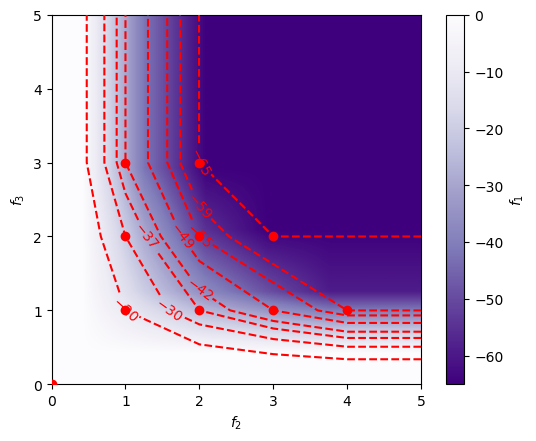
\includegraphics[width=\textwidth]{images/plot_toy_nd.png}
        \caption{Valeurs optimales de $f_1$ pour chaque $f_2$ et $f_3$. Les points rouges sont les solutions ND.}
        \label{fig:toy-nd}
    \end{subfigure}
    \hfill
    \begin{subfigure}[t]{0.49\textwidth}
        \centering
        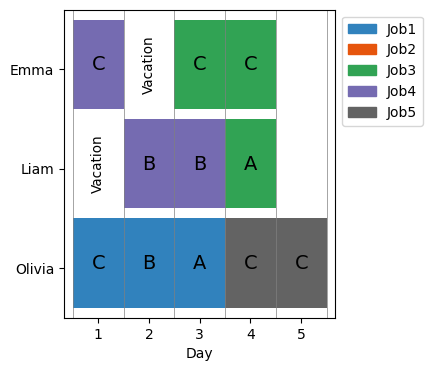
\includegraphics[width=\textwidth]{images/plot_toy_planning.png}
        \caption{Planning pour la solution ND qui minimise $f_1$ ($f_1=-65$, $f_2=2$, $f_3=3$).}
        \label{fig:toy-planning}
    \end{subfigure}
    \caption{Résultats trouvés pour l'instance << toy >>}
    \label{fig:toy}
\end{figure}    

\subsubsection{Instance << medium >>}

Pour l'instance medium, on a trouvé 46 solutions non-dominées. Des affichages similaire à celles de l'instance précédente sont montrés dans la \cref{fig:medium}. On remarque dans la \cref{fig:medium-nd} que pour la plupart des valeurs de $f_2$ et $f_3$, l'algorithme trouve la solution optimale, ce qui veut dire que si les contraintes sur le nombre maximale des projets par personne et sur la durée maximale des projets ne sont pas trop strictes, on peut toujours maximiser le gain.

\begin{figure}[H]
    \centering
    \begin{subfigure}[t]{\textwidth}
        \centering
        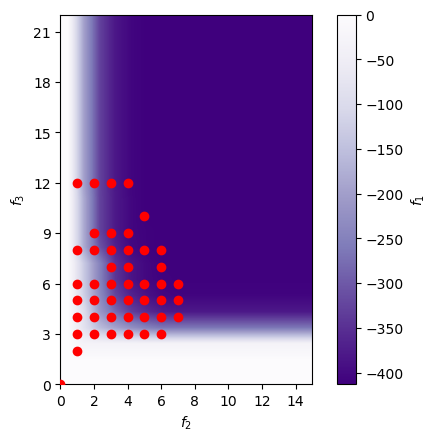
\includegraphics[width=.4\textwidth]{images/plot_medium_nd.png}
        \caption{Valeurs optimales de $f_1$ pour chaque $f_2$ et $f_3$. Les points rouges sont les solutions ND.}
        \label{fig:medium-nd}
    \end{subfigure}
    \begin{subfigure}[t]{\textwidth}
        \centering
        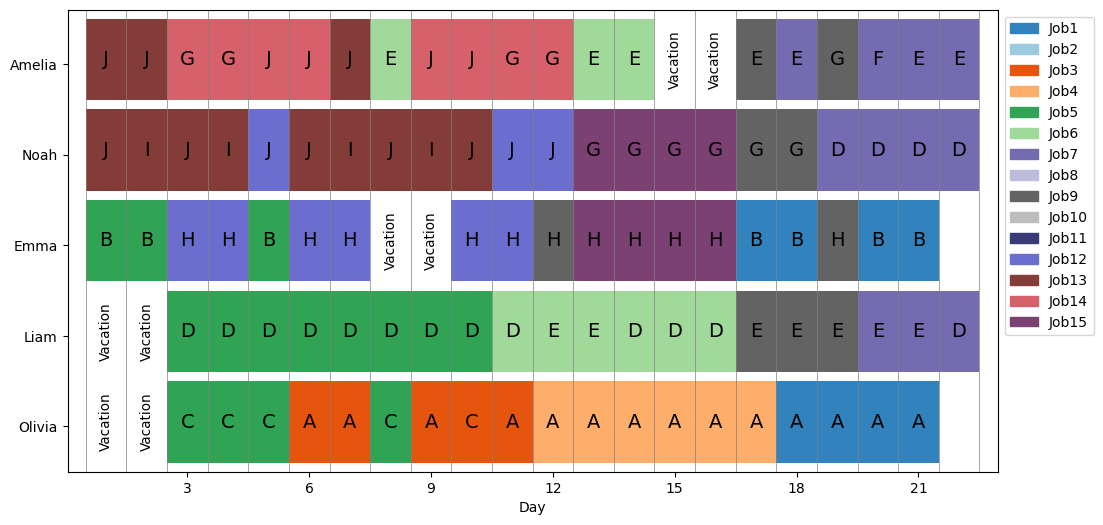
\includegraphics[width=\textwidth]{images/plot_medium_planning.png}
        \caption{Planning pour la solution ND qui minimise $f_1$ ($f_1=-413$, $f_2=5$, $f_3=10$).}
        \label{fig:medium-planning}
    \end{subfigure}
    \caption{Résultats trouvés pour l'instance << medium >>}
    \label{fig:medium}
\end{figure}

\subsubsection{Instance << large >>}
\label{sec:resultats-large}

Pour cette instance, l'optimisation était trop lente et il a fallu l'arrêter avant l'obtention des toutes les solutions optimales. Il y a donc des valeurs de $f_2$ et $f_3$ pour lesquelles la solution trouvé n'est pas optimale. Un tableau a été mis à disposition avec la solution trouvé pour chaque valeur de $f_2$ et $f_3$ (\cref{sec:tables}). Pour les cas où l'optimisation n'a pas fini, l'écart relative entre la meilleure valeur de $f_1$ trouvée et la borne de $f_1$ est donnée. Dans 20 cas, aucune solution a été trouvé dans le temps disponible.

On a ensuite utilisé cet ensemble des solutions approximatives trouvés pour obtenir les 59 solutions approximatives non dominées. Les résultats sont affichés dans la \cref{fig:large}

\begin{figure}[H]
    \centering
    \begin{subfigure}[t]{\textwidth}
        \centering
        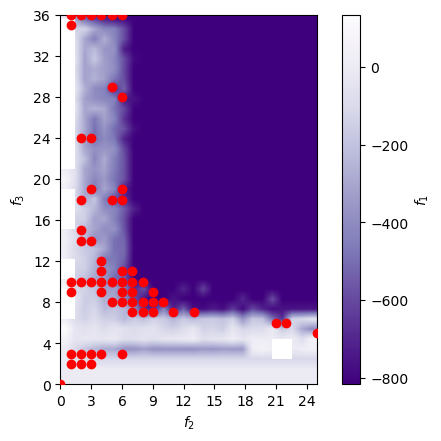
\includegraphics[width=.4\textwidth]{images/plot_large_nd.png}
        \caption{Valeurs optimales de $f_1$ pour chaque $f_2$ et $f_3$. Les points rouges sont les solutions ND.}
        \label{fig:large-nd}
    \end{subfigure}
    \begin{subfigure}[t]{\textwidth}
        \centering
        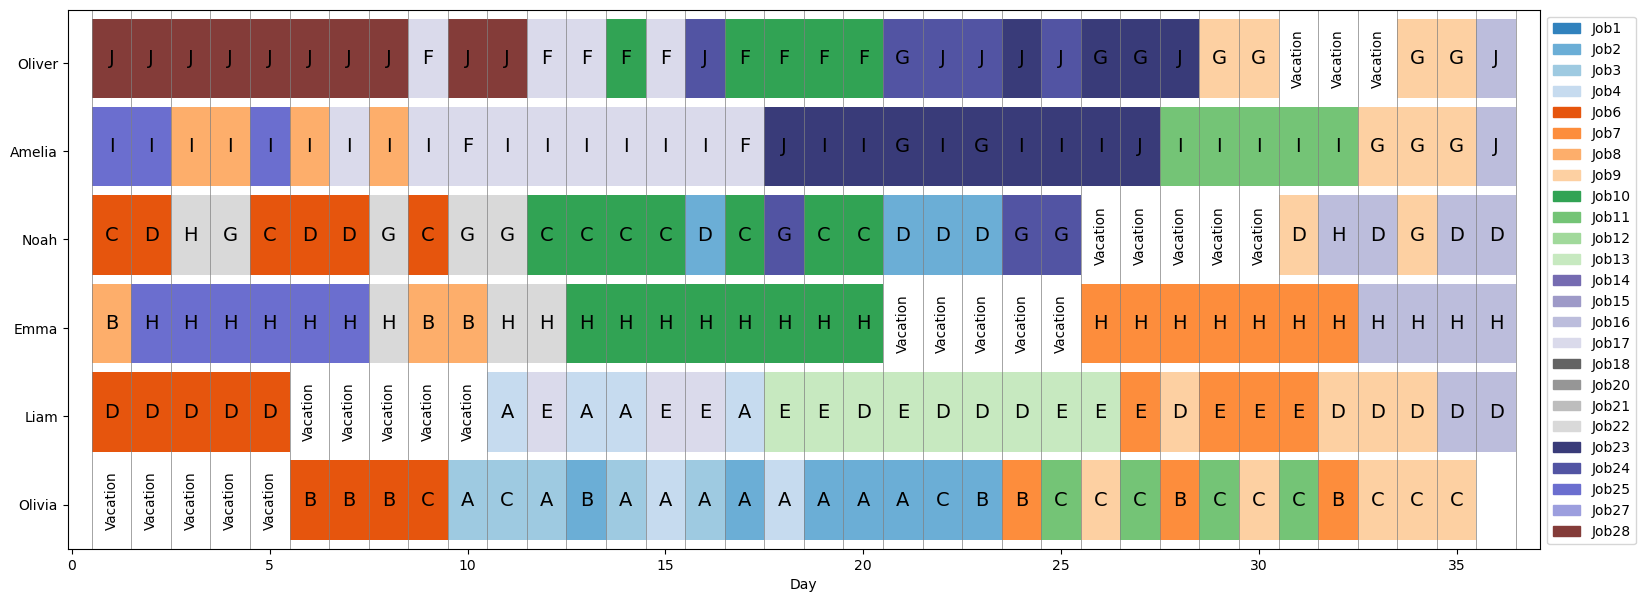
\includegraphics[width=\textwidth]{images/plot_large_planning.png}
        \caption{Planning pour la solution ND qui minimise $f_1$ ($f_1=-817$, $f_2=7$, $f_3=11$). Dans ce cas, la solution est exacte (il n'est pas possible d'avoir $f_1 < -817$}
        \label{fig:large-planning}
    \end{subfigure}
    \caption{Résultats approximatives trouvés pour l'instance << large >>}
    \label{fig:large}
\end{figure}

%%%%%%%%%%%%%%%%%%%%%%%%%%%%%%%%%%%%%%%%%%%%%%%%%%%%%%%%%%%%%%%%%%%%%%%%%%%%%%%%

\section{Modèles de préférence}

Cette seconde partie vise à développer un modèle de préférence permettant de discriminer entre les solutions de la surface des solutions non-dominées. 

Une fois que toutes les solutions non maîtrisées ont été trouvées, on entre dans un autre problème : déterminer un planning qui plaise au chef de projet et à l'administrateur. Il convient de mentionner que tous les modèles de préférences présentés ici nécessitent une sorte de préférences a priori.


\begin{figure}[H]
\centering
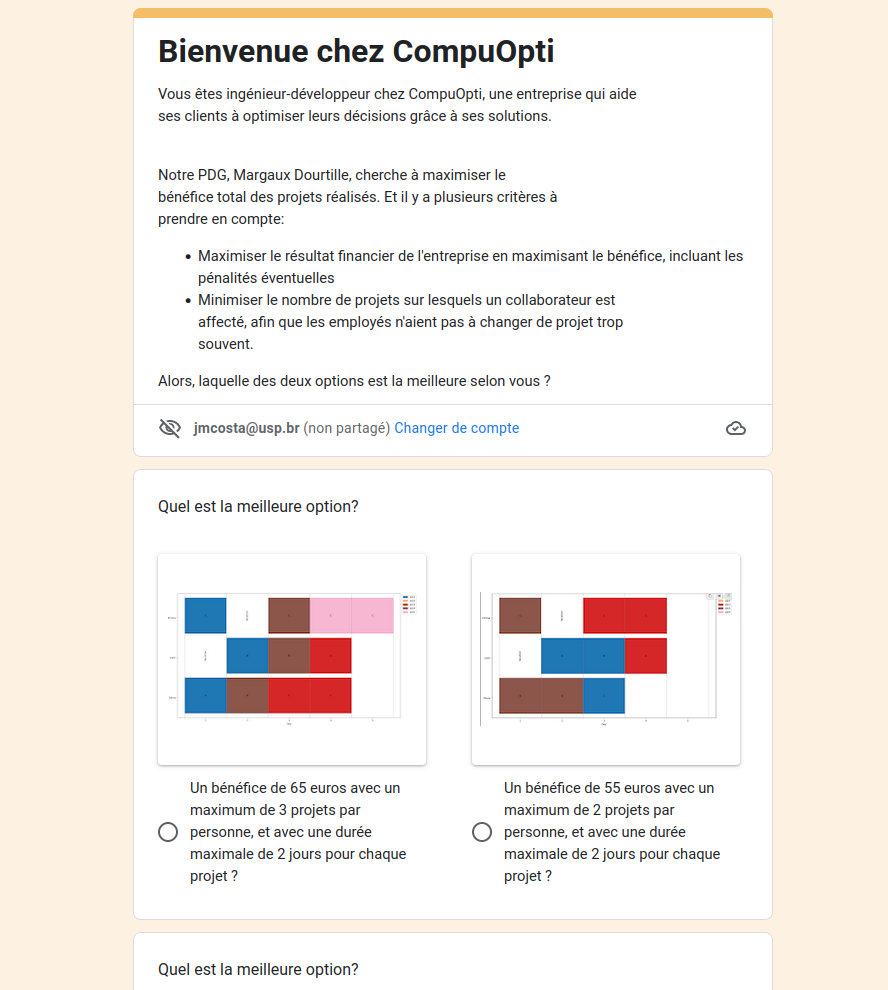
\includegraphics[width=0.6\textwidth]{images/forms.png}
\caption{Formulaires utilisés pour recueillir les préférences}
\label{fig:forms}
\end{figure}    

Compte tenu de ce qui a été présenté dans le cours, trois types de modèles ont été testés : les deux premiers sont des modèles d'agrégation, le premier considère la somme pondérée des alternatives, tandis que le second traite des fonctions de valeur additives. Enfin, une méthode de surclassement a également été testée, à travers l'implémentation de l'algorithme Promethee.

Pour obtenir les préférences, un formulaire a été créé, comme presenté para la Figure \ref{fig:forms} pour recueillir les préférences des utilisateurs, principalement pour le petit jeu d'instances (jouets). Cela a été fait uniquement pour obtenir des données sur les classements partiels ou les paires de préférences.


\subsection{UTA}

Pour ce premier problème, l'ensemble des options sont les alternatives qui constituent l'ensemble des solutions non dominées, appelé $A$. En outre, nous avons trois critères à considérer, représentés par $c = (c_1, c_2, c_3)$. Dans un premier temps, nous avons décidé d'utiliser une autre méthode classique d'agrégation pour déterminer les préférences : la combinaison de tous les critères en un seul critère appelé fonction d'utilité, $U(c) = U(c_1, c_2, c_3)$.

%Soit $P$ une relation de préférence stricte et $I$ une relation d'indifférence. Il est possible d'utiliser la valeurs d'utilité de la façon suivante :

%\begin{alignat*}{2}
%    U[c(a)] &> U[c(b)] \quad&& \text{si } aPb \\
%    U[c(a)] &= U[c(b)]      && \text{si } aIb
%\end{alignat*}
    
%Avec $c(x) = [c_1(x), c_2(x), c_3(x)]$ et $a,b \in A$.  

L'objectif de la méthode UTA est d'estimer les fonctions d'utilité en utilisant la programmation linéaire, en supposants que ces fonctions sont linéaire par morceaux.

Les entrées du programme incluentes les choix à faire et une liste indiquant les préferences. Plus précisment, dans ce cas, il est nécessaire d'avoir un ranking $R$ de taille $J$. Pour chaque critère, nous avons défini des limites et une subdivision, ce seront les valeurs minimales et maximales des données et une subdivision de 3, également espacée. De cette manière, pour chaque critère il est possible de considerer les points $c_i^k = min_i + \frac{k}{L} (max_i - min_i)$, avec $k \in \{1, 2, 3\}$. Ainsi, si une valeur est dans un intervalle on considère:

\begin{equation*}
    u_i(c_i^j)= u_i(c_i^k) + \frac{c_i^j - c_i^k}{c_i^{k+1} - c_i^k}(u_i(c_i^{k+1} - c_i^k))
\end{equation*}

En plus, pour un indice $i$, on considère $u(i) = \sum_{d}^3s_d(c_d^i) + \sigma_i$. Cette erreur est decomposée en une erreur de sous-estimation et une erreur de surestimation.


\begin{tcolorbox}

De cette manière, le problème d'optimisation était: 

\begin{equation*}
    \text{min} (\sum_j^J \sigma_j^+ + \sigma_j^-)
\end{equation*}
\textbf{Constrainte des préférences:}
\begin{alignat*}{2}
    u(i) - \sigma_i^+ + \sigma_i^- \ge s(j) - \sigma_j^+ + \sigma_j^- + \epsilon \quad \forall \text{pairs} \quad i, j \\  
\end{alignat*}

\textbf{Constrainte de monotonicité des fonctions:}
\begin{alignat*}{2}
    u_i(c_i^{k+1}) - u_i(c_i^k \ge \epsilon  \quad \forall i, k = 0 .. L_i - 1
\end{alignat*}

\textbf{Normalisation:}
\begin{alignat*}{2}
    u_i(c_i^{0})  = 0 \quad \forall i
\end{alignat*}

\begin{alignat*}{2}
  \sum_{i=1}^n \omega_i = 1 
\end{alignat*}

\end{tcolorbox}

\subsubsection{Résultats UTA}

Pour l'instance \emph{large}, en utilisant le ranking $27 \succ 8 \succ 11 \succ 7 \succ 40 \succ 12 \succ 17 \succ 53 \succ 33 \succ 34$, les résultats de cinc premiers résultats sont présentés dans le tableau \ref{tab:uta_medium} et dans la Figure \ref{fig:uta_large}

\begin{figure}[h]
\centering
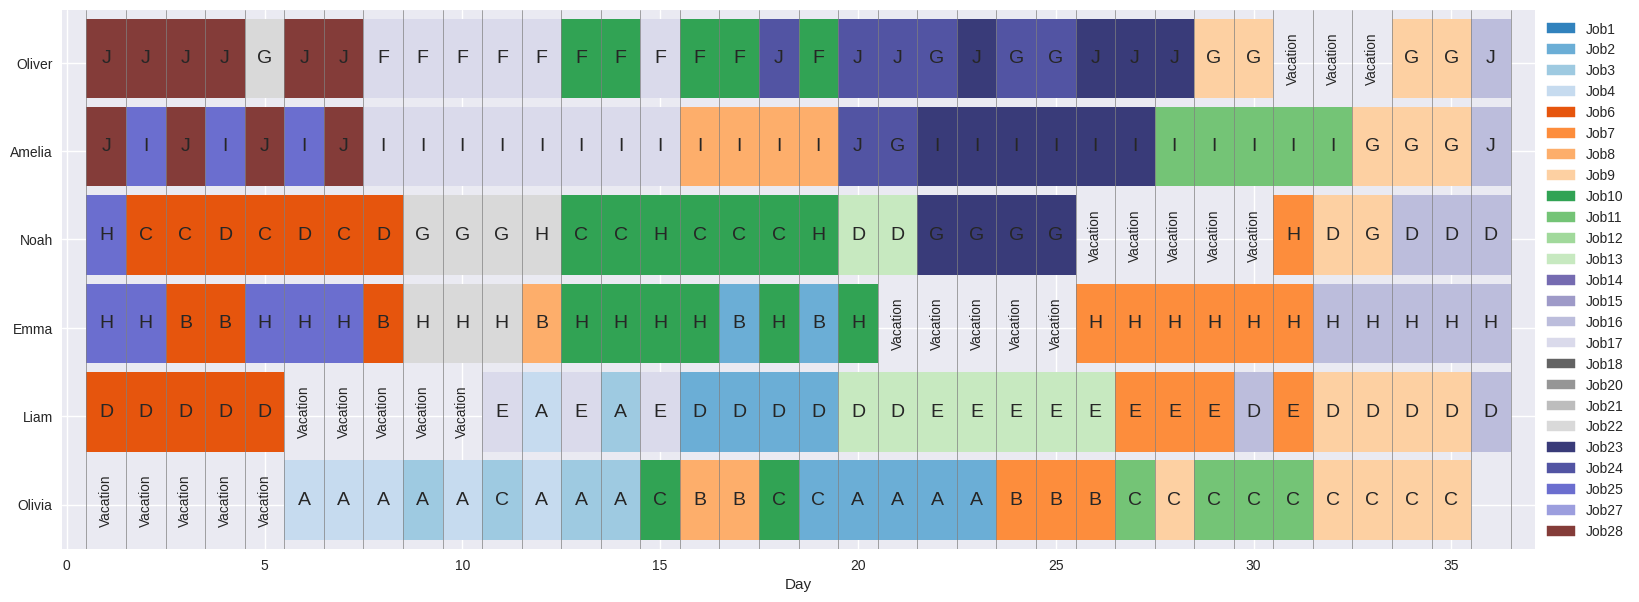
\includegraphics[width=1\textwidth]{images/best_uta_large.png}
\caption{Meilleure solution UTA - instance \emph{LARGE}}
\label{fig:uta_large_best}
\end{figure}    

\begin{table}
\centering
\begin{tabular}{c c c c c}
    \toprule
     index & $g_1$ & $g_2$ & $g_3$ & Valeur UTA \\
     \midrule
    21 & 814 & -9 & -8 & 0.108670 \\
    22 & 817 & -10 & -8 & 0.108090 \\
    34 & 814 & -7 & -10 & 0.107700 \\
    127 & 817 & -9 & -9 & 0.107605 \\
    35 & 817 & -8 & -10 & 0.1071216 \\
    \bottomrule
\end{tabular}
\caption{Valeurs classées pour l'ensemble des données \emph{medium}}
\label{tab:uta_medium}
\end{table}


Pour l'instance \emph{medium}, en utilisant le ranking $32 \succ 41 \succ 36 \succ 6 \succ 27 \succ 3 \succ 23 \succ 22 \succ 40 \succ 37$, les résultats de cinc premiers résultats sont présentés dans le tableau \ref{tab:uta_medium} et dans la Figure \ref{fig:uta_medium}


\begin{figure}[h]
\centering
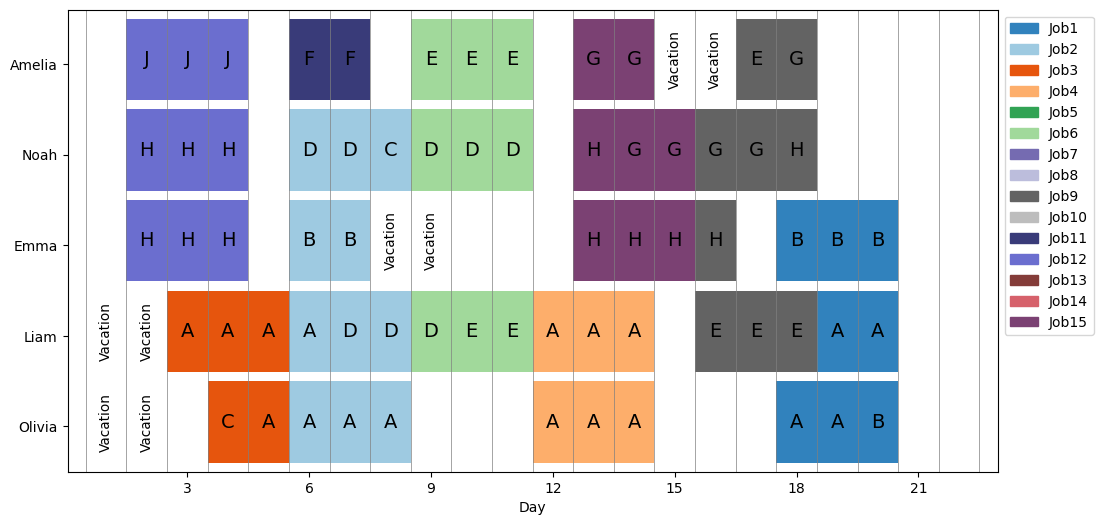
\includegraphics[width=1\textwidth]{images/best_uta_medium.png}
\caption{Meilleure solution UTA - instance \emph{medium}}
\label{fig:uta_medium_best}
\end{figure}    

\begin{table}
\centering
\begin{tabular}{c c c c c}
    \toprule
     index & $g_1$ & $g_2$ & $g_3$ & Valeur UTA \\
     \midrule
    13 & 374 & -6 & -4 & 0.112768 \\
    12 & 356 & -5 & -4 & 0.112758 \\
    19 & 389 & -5 & -5 & 0.111723 \\
    11 & 331 & -4 & -4 & 0.111632 \\
    20 & 403 & -6 & -5 & 0.111096 \\
    \bottomrule
\end{tabular}
\caption{Valeurs classées pour l'ensemble des données \emph{medium}}
\label{tab:uta_medium}
\end{table}


\begin{figure}[h]
\centering
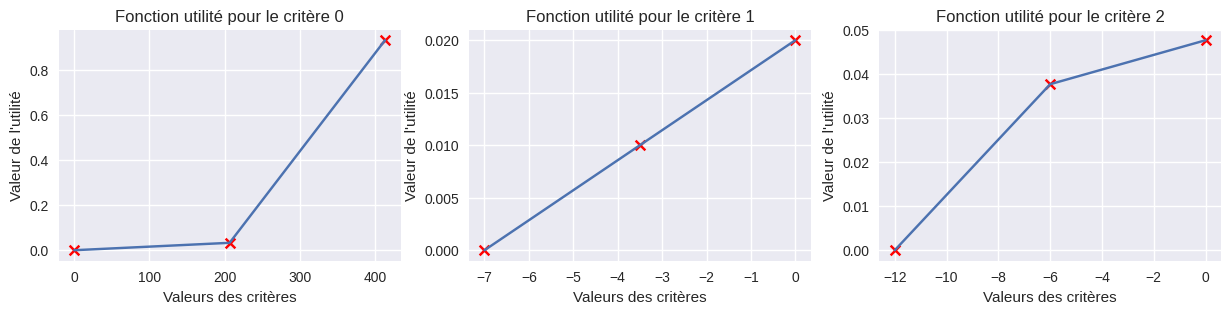
\includegraphics[width=1\textwidth]{images/uta_function.png}
\caption{Fonction utilité pour chaque critère - instance \emph{medium}}
\label{fig:uta_medium}
\end{figure}    

Pour l'instance \emph{small}, en utilisant le ranking $9 \succ 3 \succ 1$, les résultats sont présentés dans le tableau \ref{tab:uta_small} et dans la Figure \ref{fig:uta_small}

\begin{table}
\centering
\begin{tabular}{c c c c c}
    \toprule
     index & $g_1$ & $g_2$ & $g_3$ & Valeur UTA \\
     \midrule
    7 & 65.0 & -3.0 & -2.0 & 1.911667 \\
    9 & 65.0 & -2.0 & -3.0 & 1.910000 \\
    4 & 59.0 & -4.0 & -1.0 & 1.737949 \\
    6 & 55.0 & -2.0 & -2.0 & 1.624359 \\
    3 & 49.0 & -3.0 & -1.0 & 1.450641 \\
    8 & 42.0 & -1.0 & -3.0 & 1.242692 \\
    2 & 37.0 & -2.0 & -1.0 & 1.104872 \\
    5 & 30.0 & -1.0 & -2.0 & 0.898590 \\
    1 & 20.0 & -1.0 & -1.0 & 0.612949 \\
    0 & -0.0 & -0.0 & -0.0 & 0.040000 \\
    \bottomrule
\end{tabular}
\caption{Valeurs classées pour l'ensemble des données \emph{small}}
\label{tab:uta_small}
\end{table}


\begin{figure}[H]
\centering
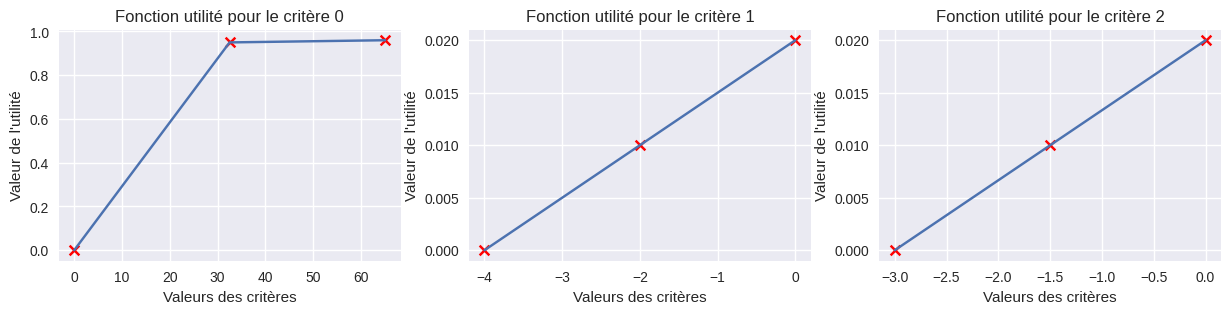
\includegraphics[width=1\textwidth]{images/uta_small.png}
\caption{Fonction utilité pour chaque critère - instance \emph{small}}
\label{fig:uta_small}
\end{figure}    


\begin{figure}[H]
\centering
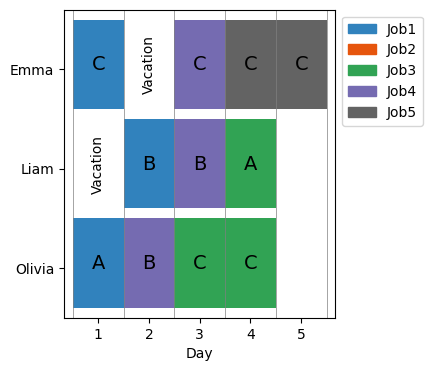
\includegraphics[width=0.5\textwidth]{images/best_uta_small.png}
\caption{Meilleure solution UTA - instance \emph{small}}
\label{fig:uta_small}
\end{figure}    


\subsection{Somme ponderée}

La méthode de la somme pondérée est une approche couramment utilisée dans l'analyse décisionnelle multicritères (MCDA), problablement la plus simple à conceptualiser. Comme dans la méthode précedente, dans cette méthode, l'ensemble d'alternatives (solutions non dominées) est évalué sur la base de trois critères, qui sont combinés en une unique valeur.

Dans ce cas, les critères sont pondérés pour refléter leur importance relative, et les valeurs des alternatives pour chaque critère sont multipliées par leurs poids respectifs pour calculer un score total pondéré, comme presenté par l'équation \ref{eq:sommep}. Ce score représente l'évaluation globale de chaque alternative, et le décideur peut choisir l'alternative ayant le score le plus élevé comme option préférée. La méthode de la somme pondérée est simple, intuitive et facile à utiliser, mais elle a ses limites car elle suppose que les critères sont indépendants et de même poids.

\begin{equation*}
U(g^k) = \sum_{i=1}^3 \omega_i * g_i^k    
\label{eq:sommep}
\end{equation*}

En outre, certaines contraintes de normalisation ont été fixées, commenté ci-dessous.

\begin{tcolorbox}

\textbf{Pour chaque paire:}
\begin{alignat*}{2}
    i \succ j \rightarrow \omega_1(g^i_1 - g^j_1) + \omega_2(g^i_2 - g^j_2) + \omega_3(g^i_3 - g^j_3) \ge 0
 \end{alignat*}

\textbf{Normalisation:}
\begin{alignat*}{3}
    \sum_{i=1}^n \omega_i = 1 
\end{alignat*}
\end{tcolorbox}


Le problème d'optimisation à résoudre consiste à rechercher des vecteurs de poids dans l'espace défini par les contraintes. Une fois les relations de dominance trouvées, il est possible de créer une pré-commande, comme le montre le graphe \ref{fig:graph+somme_ponderee}.

\begin{figure}[H]
\centering
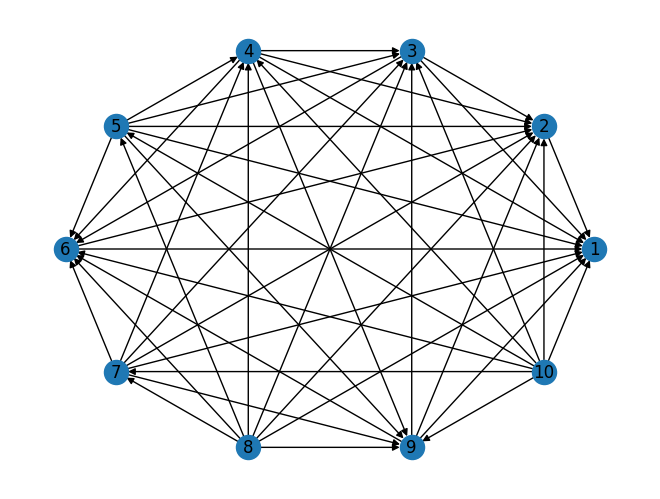
\includegraphics[width=0.7\textwidth]{images/graph_small_somme_ponderee.png}
\caption{Graphe Somme ponderée - instance \emph{small}}
\label{fig:graph+somme_ponderee}
\end{figure}    

La valeur permettant de classer les alternatives, cependant, a été calculée en tenant compte du degré de sortie moins le degré d'entrée de chaque nœud du graphe.

\subsubsection{Résultats - somme ponderée}

Pour l'instance \emph{large}, les preférences utilisées étaient $(27 \succ 3), (27 \succ 4),  (27 \succ 55),  (57 \succ 56),  (58 \succ 52),  (58 \succ 3),  (57 \succ 8),  (58 \succ 2),  (23 \succ 28),  (4 \succ 5),  (21 \succ 27),  (35 \succ 27),  (35 \succ 38), (21 \succ 34)$. Les résultats des cinc premiers éléments sont présentés dans le tableau \ref{tab:somme_pond_large} et le planning final est presenté dans la Figure \ref{fig:best_somme_ponderee_large}.

\begin{table}[htbp]
\centering
\begin{tabular}{c c c c c}
\toprule
index & $g_1$ & $g_2$ & $g_3$ & degree \\
\midrule
22 & 817 & -10 & -8 & 56 \\
27 & 817 & -9 & -9 & 54 \\
31 & 814 & -9 & -8 & 54 \\
35 & 817 & -8 & -10 & 52 \\
34 & 814 & -7 & -10 & 52 \\
\bottomrule
\end{tabular}
\caption{Valeurs classées pour l’ensemble des données \emph{medium}}
\label{tab:somme_pond_large}
\end{table}


\begin{figure}[H]
\centering
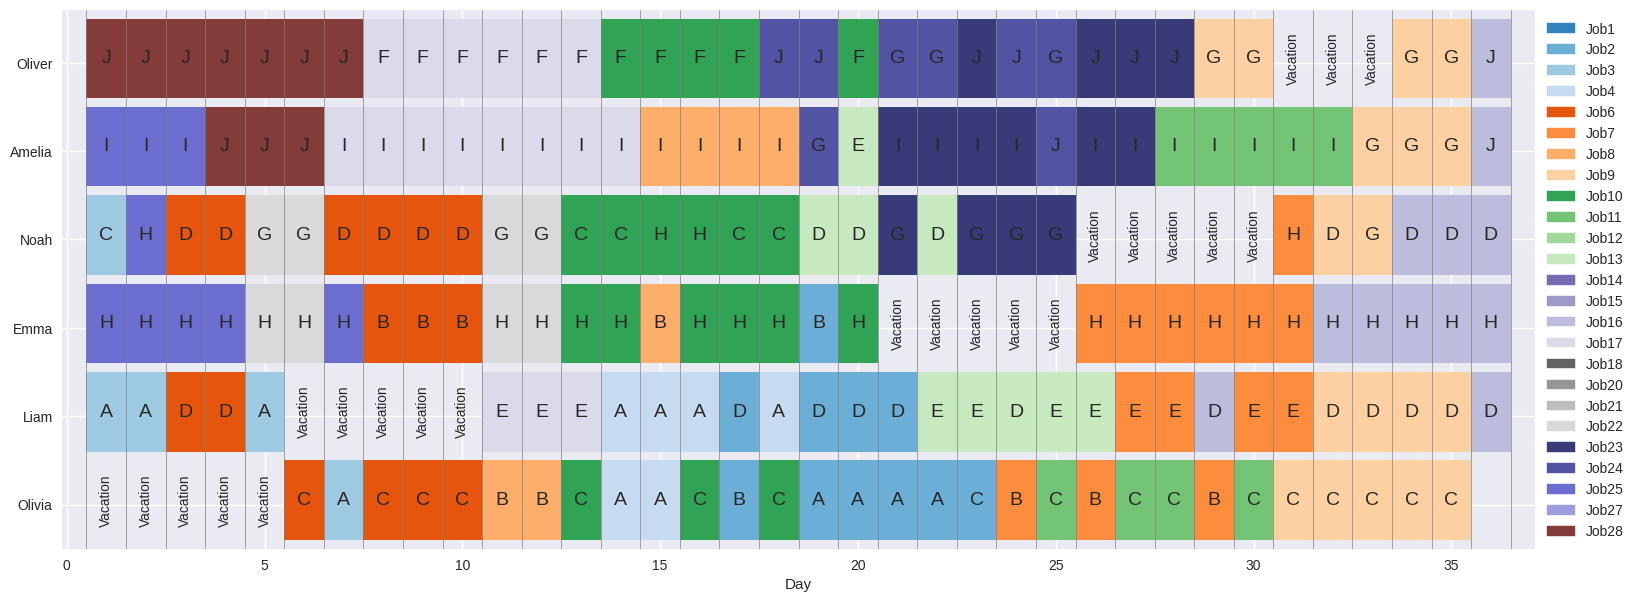
\includegraphics[width=1\textwidth]{images/best_somme_pondere_large.png}
\caption{Meilleure solution somme ponderee - instance \emph{large}}
\label{fig:best_somme_ponderee_large}
\end{figure}    



Pour l'instance \emph{medium}, les preférences utilisées étaient $(9 \succ 3), (9 \succ 1), (12 \succ 7), (30 \succ 6), (31 \succ 35), (3 \succ 1), (40 \succ  30)$. Les résultats des cinc premiers éléments sont présentés dans le tableau \ref{tab:somme_pond_medium}.


\begin{table}[htbp]
\centering
\begin{tabular}{c c c c c}
\toprule
index & $g_1$ & $g_2$ & $g_3$ & degree \\
\midrule
27 & 408 & -6 & -6 & 37 \\
26 & 403 & -5 & -6 & 35 \\
36 & 410 & -5 & -8 & 34 \\
20 & 403 & -6 & -5 & 34 \\
28 & 411 & -7 & -6 & 34 \\
\bottomrule
\end{tabular}
\caption{Valeurs classées pour l’ensemble des données \emph{medium}}
\label{tab:somme_pond_medium}
\end{table}


\begin{figure}[H]
\centering
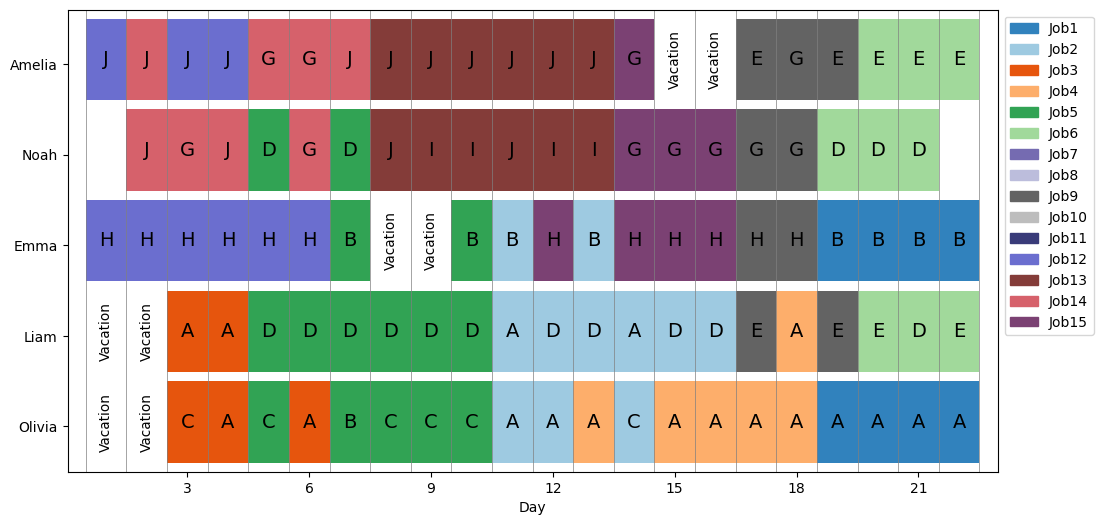
\includegraphics[width=1\textwidth]{images/best_somme_pondere_medium.png}
\caption{Meilleure solution somme ponderee - instance \emph{medium}}
\label{fig:best_somme_ponderee_medium}
\end{figure}    

Pour l'instance \emph{small}, en utilisant les preférences $9 \succ 3$, $9 \succ 1$ et $3 \succ 1$, les résultats sont présentés dans le tableau \ref{tab:somme_pond_small}.


\begin{table}[htbp]
\centering
\begin{tabular}{c c c c c}
\toprule
index & $g_1$ & $g_2$ & $g_3$ & degree \\
\midrule
8 & 65.0 & -3.0 & -2.0 & 8 \\
10 & 65.0 & -2.0 & -3.0 & 8 \\
5 & 59.0 & -4.0 & -1.0 & 4 \\
7 & 55.0 & -2.0 & -2.0 & 4 \\
4 & 49.0 & -3.0 & -1.0 & 1 \\
9 & 42.0 & -1.0 & -3.0 & -1 \\
3 & 37.0 & -2.0 & -1.0 & -3 \\
6 & 30.0 & -1.0 & -2.0 & -5 \\
2 & 20.0 & -1.0 & -1.0 & -7 \\
1 & -0.0 & -0.0 & -0.0 & -9 \\ 
\bottomrule
\end{tabular}
\caption{Valeurs classées pour l’ensemble des données \emph{small}}
\label{tab:somme_pond_small}
\end{table}



\subsection{PROMETHEE I}

En outre des méthodes d'aggrégation, un autre experiment était l'utilisation d'une méthode de surclassement. Ces méthodes, comme Promethee, sont utilisées pour l'enrichissement des évaluations et son complément descriptif analyse géométrique pour l'aide interactive. Fondamentalement, ces méthodes peuvent nous aider à prendre des décisions en déterminant quelle option est la plus adaptée à nos objectifs et à la compréhension du problème. Au lieu de nous dire la "bonne" réponse, la méthode Promethee nous offre un cadre complet et rationnel pour prendre une décision.

Au début, il est nécessaire de fournir un vecteur de poids, défini par le décideur, et des paramètres pour les fonctions qui modelisent les critères. En ce qui concerne les choix faites, les poids utilisées étaient ceux sortis de la méthode de somme ponderé. Les préférences étaient modélisés avec une fonction gaussienne, c'est-à-dire:

\begin{equation}
    P(a, b) = f(d) = 1 - exp(-\frac{d^2}{2\sigma^2})
\end{equation}

où, $d = a - b$ et $\sigma$ sont les paramètres fournis pour chaque critère.

La méthode consiste en créer une matrice $\mathbb{R}^{N_s, N_f}$, où $N_s$ est le nombre de solutions et $N_f$ est le nombre de critères. Après la méthode calcule la distance de chaque solution par chaque critère : D = \{$d \in \mathbb{R}^{N_s,N_s,N_f} : d_k(s_i, s_j) = f_k(s_i) - f_k(s_j)$ \}. Ensuite, appliquer la fonction gaussienne et multiplier pour les poids. Finalement, les scores sont calculées en fonction du flux de sortie et d'éntrée.


\subsubsection{Résultats - PROMETHEE}

Pour l'instance \emph{small}, les paramètres utilisés étaient $W = [0.07 0.5 0.43]$ pour les poids, $S = [20, 1, 2]$ pour les fonctions gaussiennes. Les résultats sont présentés dans la Figure \ref{fig:graph+somme_ponderee}.

\begin{figure}[H]
\centering
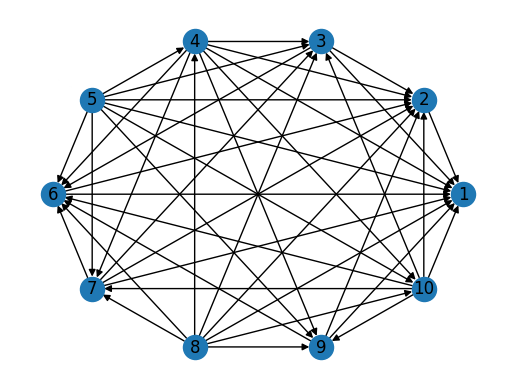
\includegraphics[width=0.7\textwidth]{images/promethee_graph.png}
\caption{Graphe Promethee - instance \emph{small}}
\label{fig:graph+somme_ponderee}
\end{figure}    


\begin{figure}[H]
\centering
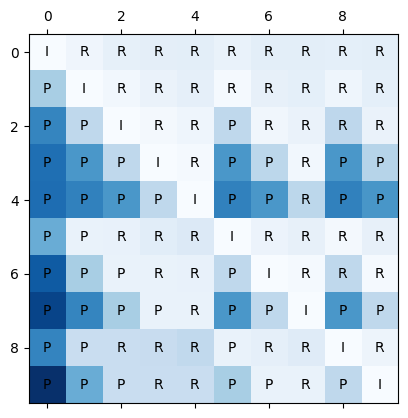
\includegraphics[width=0.5\textwidth]{images/promethee_preference_matrix.png}
\caption{Matrice de préférences - instance \emph{small}}
\label{fig:graph+somme_ponderee}
\end{figure}    


%%%%%%%%%%%%%%%%%%%%%%%%%%%%%%%%%%%%%%%%%%%%%%%%%%%%%%%%%%%%%%%%%%%%%%%%%%%%%%%%

\section{Conclusion}

Ce document montre l'implémentation de l'optimisation pour trois instances en utilisant la librarie Gurobi. La méthode utilisée consiste à parcourir les combinaisons de $f_2$ et $f_3$ et à optimiser $f_1$ pour chacune d'entre elles pour trouver les solutions non dominées. La feature multi-scénario de Gurobi a été utilisée pour réduire les délais d'optimisation. Des solutions non-dominées ont été trouvées pour l'instance la plus petite, avec un total de 10 solutions. Les résultats sont affichés sous forme de diagrammes pour montrer les travaux effectués par personne, compétence et jour, ainsi que la relation entre les trois fonctions objectives et les solutions non-dominées. Les prochains pas pourraient inclure une vérification plus approfondie des résultats et une évaluation des performances pour les deux autres instances.

Finalement, la seconde partie de ce document a cherché à développer un modèle de préférence pour discriminer les solutions de la surface des solutions non-dominées. Pour cela, trois types de modèles ont été testés, à savoir les modèles d'agrégation pondérés et les fonctions de valeur additives, ainsi qu'une méthode de surclassement à travers l'algorithme Promethee. Pour obtenir les préférences, un formulaire a été créé pour recueillir les données des utilisateurs. Le premier modèle UTA testé implique une estimation des fonctions d'utilité à l'aide de la programmation linéaire en supposant que ces fonctions sont linéaires par morceaux. Bien que les résultats semblent prometteurs, il est important de noter que la méthode UTA nécessite des données préliminaires sur les préférences des utilisateurs. Les prochains pas incluent la continuation de l'application de ces modèles à des jeux de données plus importants et plus complexes, ainsi que l'analyse des résultats pour évaluer leur pertinence pour résoudre ce type de problème.

\clearpage
\appendix

\section{Tableaux des Résultats}
\label{sec:tables}

\begin{table}[H]
    \centering
    \begin{tabular}{r r r}
        \toprule
        $f_1$ & $f_2$ & $f_3$ \\
        \midrule
          0 & 0 & 0 \\
        -20 & 1 & 1 \\
        -37 & 2 & 1 \\
        -49 & 3 & 1 \\
        -59 & 4 & 1 \\
        -30 & 1 & 2 \\
        -55 & 2 & 2 \\
        -65 & 3 & 2 \\
        -42 & 1 & 3 \\
        -65 & 2 & 3 \\
        \bottomrule
    \end{tabular}
    \caption{Solutions non-dominées pour l'instance << toy >>}
\end{table}

\begin{table}[H]
    \centering
    \begin{tabular}{r r r}
        \toprule
        $f_1$ & $f_2$ & $f_3$ \\
        \midrule
           0 & 0 & 0 \\
         -30 & 1 & 2 \\
         -80 & 1 & 3 \\
        -155 & 2 & 3 \\
        -195 & 3 & 3 \\
        -225 & 4 & 3 \\
        -250 & 5 & 3 \\
        -265 & 6 & 3 \\
         -90 & 1 & 4 \\
        -210 & 2 & 4 \\
        -279 & 3 & 4 \\
        -331 & 4 & 4 \\
        \bottomrule
    \end{tabular}
    \hspace*{1cm}
    \begin{tabular}{r r r}
        \toprule
        $f_1$ & $f_2$ & $f_3$ \\
        \midrule
        -356 & 5 & 4 \\
        -374 & 6 & 4 \\
        -380 & 7 & 4 \\
        -120 & 1 & 5 \\
        -232 & 2 & 5 \\
        -322 & 3 & 5 \\
        -365 & 4 & 5 \\
        -389 & 5 & 5 \\
        -403 & 6 & 5 \\
        -406 & 7 & 5 \\
        -130 & 1 & 6 \\
        -245 & 2 & 6 \\
        \bottomrule
    \end{tabular}
    \hspace*{1cm}
    \begin{tabular}{r r r}
        \toprule
        $f_1$ & $f_2$ & $f_3$ \\
        \midrule
        -343 & 3 & 6 \\
        -385 & 4 & 6 \\
        -403 & 5 & 6 \\
        -408 & 6 & 6 \\
        -411 & 7 & 6 \\
        -346 & 3 & 7 \\
        -386 & 4 & 7 \\
        -411 & 6 & 7 \\
        -180 & 1 & 8 \\
        -305 & 2 & 8 \\
        -370 & 3 & 8 \\
        \bottomrule\\
    \end{tabular}
    \hspace*{1cm}
    \begin{tabular}{r r r}
        \toprule
        $f_1$ & $f_2$ & $f_3$ \\
        \midrule
        -401 & 4 & 8 \\
        -410 & 5 & 8 \\
        -413 & 6 & 8 \\
        -325 & 2 & 9 \\
        -379 & 3 & 9 \\
        -404 & 4 & 9 \\
        -413 & 5 & 10 \\
        -194 & 1 & 12 \\
        -326 & 2 & 12 \\
        -382 & 3 & 12 \\
        -405 & 4 & 12 \\
        \bottomrule\\
    \end{tabular}
    \caption{Solutions non-dominées pour l'instance << medium >>}
\end{table}

\begin{table}[H]
    \centering
    \begin{tabular}{r r r r}
        \toprule
        $f_1$ & $f_2$ & $f_3$ & écart ($\%$) \\
        \midrule
           0 &  0 &  0           \\
         -60 &  1 &  2           \\
         -90 &  2 &  2 &  53.3\% \\
        -115 &  3 &  2 & 173.9\% \\
         -90 &  1 &  3           \\
        -185 &  2 &  3 &  77.3\% \\
        -235 &  3 &  3 & 107.2\% \\
        -290 &  4 &  3 & 106.6\% \\
        -370 &  6 &  3 &  93.2\% \\
        -399 & 25 &  5 & 104.8\% \\
        -482 & 21 &  6 &  69.5\% \\
        -674 & 22 &  6 &  21.2\% \\
        -373 &  7 &  7 & 119.0\% \\
        -687 &  8 &  7 &  18.9\% \\
        -707 &  9 &  7 &  15.6\% \\
        -737 & 11 &  7 &  10.9\% \\
        -782 & 13 &  7 &   4.5\% \\
        -304 &  5 &  8 & 168.8\% \\
        -415 &  6 &  8 &  96.9\% \\
        -571 &  7 &  8 &  43.1\% \\
        -751 &  8 &  8 &   8.8\% \\
        -814 &  9 &  8 &   0.4\% \\
        -817 & 10 &  8           \\
        -112 &  1 &  9 & 629.5\% \\
        -332 &  4 &  9 & 146.1\% \\
        -433 &  6 &  9 &  88.7\% \\
        -681 &  7 &  9 &  20.0\% \\
        -817 &  9 &  9           \\
        -132 &  1 & 10 & 518.9\% \\
        -207 &  2 & 10 & 294.7\% \\
        \bottomrule
    \end{tabular}
    \hspace*{1cm}
    \begin{tabular}{r r r r}
        \toprule
        $f_1$ & $f_2$ & $f_3$ & écart ($\%$) \\
        \midrule
        -303 &  3 & 10 & 169.6\% \\
        -359 &  4 & 10 & 127.6\% \\
        -514 &  5 & 10 &  58.9\% \\
        -534 &  6 & 10 &  53.0\% \\
        -814 &  7 & 10 &   0.4\% \\
        -817 &  8 & 10           \\
        -372 &  4 & 11 & 119.6\% \\
        -597 &  6 & 11 &  36.9\% \\
        -817 &  7 & 11           \\
        -463 &  4 & 12 &  76.5\% \\
        -221 &  2 & 14 & 269.7\% \\
        -392 &  3 & 14 & 108.4\% \\
        -237 &  2 & 15 & 244.7\% \\
        -297 &  2 & 18 & 175.1\% \\
        -587 &  5 & 18 &  39.2\% \\
        -667 &  6 & 18 &  22.5\% \\
        -472 &  3 & 19 &  73.1\% \\
        -723 &  6 & 19 &  13.0\% \\
        -327 &  2 & 24 & 149.8\% \\
        -496 &  3 & 24 &  64.7\% \\
        -747 &  6 & 28 &   9.4\% \\
        -676 &  5 & 29 &  20.9\% \\
        -143 &  1 & 35 & 471.3\% \\
        -290 &  1 & 36           \\
        -510 &  2 & 36 &  19.0\% \\
        -626 &  3 & 36 &  16.8\% \\
        -708 &  4 & 36 &  11.2\% \\
        -764 &  5 & 36 &   6.9\% \\
        -779 &  6 & 36 &   4.9\% \\
        \bottomrule\\
    \end{tabular}
    \caption{Solutions non-dominées pour l'instance << large >>. Pour le solutions qui ne sont pas forcement optimales l'écart relatif d'optimalité à la fin de l'optimisation est indiqué (c.f. \cref{sec:resultats-large}).}
\end{table}

\end{document}
    